\documentclass{article}[18pt]
\ProvidesPackage{format}
%Page setup
\usepackage[utf8]{inputenc}
\usepackage[margin=0.7in]{geometry}
\usepackage{parselines} 
\usepackage[english]{babel}
\usepackage{fancyhdr}
\usepackage{titlesec}
\hyphenpenalty=10000

\pagestyle{fancy}
\fancyhf{}
\rhead{Sam Robbins}
\rfoot{Page \thepage}

%Characters
\usepackage{amsmath}
\usepackage{amssymb}
\usepackage{gensymb}
\newcommand{\R}{\mathbb{R}}

%Diagrams
\usepackage{pgfplots}
\usepackage{graphicx}
\usepackage{tabularx}
\usepackage{relsize}
\pgfplotsset{width=10cm,compat=1.9}
\usepackage{float}

%Length Setting
\titlespacing\section{0pt}{14pt plus 4pt minus 2pt}{0pt plus 2pt minus 2pt}
\newlength\tindent
\setlength{\tindent}{\parindent}
\setlength{\parindent}{0pt}
\renewcommand{\indent}{\hspace*{\tindent}}

%Programming Font
\usepackage{courier}
\usepackage{listings}
\usepackage{pxfonts}

%Lists
\usepackage{enumerate}
\usepackage{enumitem}

% Networks Macro
\usepackage{tikz}


% Commands for files converted using pandoc
\providecommand{\tightlist}{%
	\setlength{\itemsep}{0pt}\setlength{\parskip}{0pt}}
\usepackage{hyperref}

% Get nice commands for floor and ceil
\usepackage{mathtools}
\DeclarePairedDelimiter{\ceil}{\lceil}{\rceil}
\DeclarePairedDelimiter{\floor}{\lfloor}{\rfloor}

% Allow itemize to go up to 20 levels deep (just change the number if you need more you madman)
\usepackage{enumitem}
\setlistdepth{20}
\renewlist{itemize}{itemize}{20}

% initially, use dots for all levels
\setlist[itemize]{label=$\cdot$}

% customize the first 3 levels
\setlist[itemize,1]{label=\textbullet}
\setlist[itemize,2]{label=--}
\setlist[itemize,3]{label=*}

% Definition and Important Stuff
% Important stuff
\usepackage[framemethod=TikZ]{mdframed}

\newcounter{theo}[section]\setcounter{theo}{0}
\renewcommand{\thetheo}{\arabic{section}.\arabic{theo}}
\newenvironment{important}[1][]{%
	\refstepcounter{theo}%
	\ifstrempty{#1}%
	{\mdfsetup{%
			frametitle={%
				\tikz[baseline=(current bounding box.east),outer sep=0pt]
				\node[anchor=east,rectangle,fill=red!50]
				{\strut Important};}}
	}%
	{\mdfsetup{%
			frametitle={%
				\tikz[baseline=(current bounding box.east),outer sep=0pt]
				\node[anchor=east,rectangle,fill=red!50]
				{\strut Important:~#1};}}%
	}%
	\mdfsetup{innertopmargin=10pt,linecolor=red!50,%
		linewidth=2pt,topline=true,%
		frametitleaboveskip=\dimexpr-\ht\strutbox\relax
	}
	\begin{mdframed}[]\relax%
		\centering
		}{\end{mdframed}}



\newcounter{lem}[section]\setcounter{lem}{0}
\renewcommand{\thelem}{\arabic{section}.\arabic{lem}}
\newenvironment{defin}[1][]{%
	\refstepcounter{lem}%
	\ifstrempty{#1}%
	{\mdfsetup{%
			frametitle={%
				\tikz[baseline=(current bounding box.east),outer sep=0pt]
				\node[anchor=east,rectangle,fill=blue!20]
				{\strut Definition};}}
	}%
	{\mdfsetup{%
			frametitle={%
				\tikz[baseline=(current bounding box.east),outer sep=0pt]
				\node[anchor=east,rectangle,fill=blue!20]
				{\strut Definition:~#1};}}%
	}%
	\mdfsetup{innertopmargin=10pt,linecolor=blue!20,%
		linewidth=2pt,topline=true,%
		frametitleaboveskip=\dimexpr-\ht\strutbox\relax
	}
	\begin{mdframed}[]\relax%
		\centering
		}{\end{mdframed}}
\lhead{Computational Thinking}
\begin{document}
\begin{center}
\underline{\huge What is Computer Software?}
\end{center}
\textbf{Algorithm} - Sequences of precise instructions that can be applied to data items\\
\textbf{Programming Language}  - A means for translating an algorithm into a form suitable for execution by a computer. Into a program that can then be translated into a form suitable for execution by a computer.\\
\\
An algorithm is not a computer program
\begin{itemize}
\item Program is written in a programming language
\item There are an infinite number of \textbf{implementations} of algorithms as programs
\end{itemize}
\section{Programming languages}
Programming languages can be of different \textbf{programming paradigms}:
\begin{itemize}
\item Imperative - Statements change a programs \textbf{state} (closest to "memory abstraction" of CPU) (Python, C++, Java etc) - Take data, do operation on it, then write that data back to memory
\item Declarative  - Programs say \textbf{what} rather than \textbf{how} - Lack flow control: loops, if statements etc
\begin{itemize}
\item Functional - Programs are defined as "mathematical" functions (don't have standard set of syntax: if etc). To get an answer build up a large functional expression that gives the correct output given an input
\item Logic - Programs specify a "logical solution" - input rules and known information, then ask a question
\end{itemize}
\item Data-oriented - Programs work with data through manipulating and searching relations (tables). Tables have things in common that can be linked together to get more information. 
\item Scripting - Designed to automate frequently used tasks that involve calling or passing commands to external programs. These languages have lots of libraries to make things easier to do
\item Object Oriented - Small piece of code relating to a particular object (person etc) create instances of object with different information, link these together
\end{itemize}
More rare types:
\begin{itemize}
\item Assembly - Low level languages providing the interface between machine code and a high-level programming language. Faster as closer to what the machine processes so less overhead
\item Concurrent - Provides facilities for concurrency (threads, processes); may be \textbf{message-passing} or \textbf{shared-memory}. 
\item Dataflow - Programs specified by flows of data (usually visual, like a flowchart)
\item Fourth-generation - High level languages built around databases
\item List based - Built around list data structure
\item Visual - Allows user to specify programs using visual representations
\end{itemize}
\subsection{Why more and more languages}
Programming language design has been driven by
\begin{itemize}
\item Productivity
\begin{itemize}
\item C++, Java etc
\item Expensive to develop/maintain
\item Rapid application development (RAD) languages - quicker to make, quicker to sell, quicker to make money
\end{itemize}
\item Reliability 
\begin{itemize}
\item Features to enhance error detection (type checking etc)
\item Aliasing - 2 variables referring to the same piece of data, at some time change the value of one of the variables. This changes the other value also
\end{itemize}
\item Security
\begin{itemize}
\item Do we trust programming languages? - Using these languages to send bank detauls etc
\end{itemize}
\item Execution speed
\begin{itemize}
\item Imperative languages are not tied to sequential computers
\item Not to parallel/distributed computers
\item Need speed for medical, scientific etc
\end{itemize}
\item Curiosity and style
\end{itemize}
\subsection{Programming languages should}
\begin{itemize}
\item Be easy to use,read and write (collaborate)
\item Support abstraction (adding new features)
\item Support testing, debugging and verification
\item Be inexpensive to use and maintain
\end{itemize}
\subsection{Logic Programming}
\begin{itemize}
\item Dates back to the late fifties
\item Uses mathematical logic to "compute"
\item Learn more and more until you know the answer to a question
\end{itemize}
Logic is used
\begin{itemize}
\item Procedurally - Rule
\item Declaratively  - Input
\end{itemize}
Incorporating logic procedurally and declaratively allows us to "compute"\\
\\
Programs come in 2 parts
\begin{itemize}
\item The program - Things you know and a list of rules
\item The query - What do you want to learn?
\end{itemize}
\subsubsection{Example prolog program}
\begin{itemize}
\item Start with a list of facts (full stop terminates a fact)
\item Add some rules (Underscore is a wildcard) (use commas as and to allow for more complicated rules)
\end{itemize}
\begin{lstlisting}[mathescape=true,language=Prolog]
female(artemis).
female(persephone).
male(apollo).
mother(gia,uranus).
parents(uranus,gaia,rhea).
parents(cronus,rhea,zeus).
parents(cronus,rhea,hera).
parents(cronus,rhea,demeter).
parents(zeus,leto, artemis).
parents(zeus,leto,apollo).
parents(zeus,hera,hebe).
parents(demeter,zeus,persephone).
%rules
mother(X,Y):-parents(_,X,Y).
female(X):-mother(X,_). %If a person is the mother of anybody, they are female
father(X,Y):-parents(X,_,Y)
%These rules can be continued to make other rules about families
%Query
?- mother(gia,zeus).
no
\end{lstlisting}


\section{Research Glimpse - Parallel Computing}
Programming in parallel\\
Why should we program in parallel
\begin{itemize}
\item Performance - speedup when using all cores
\item Hiding latency (e.g. slow IO) (keep doing instructions until information received)
\item Real world concurrency (lots of people able to use a service)
\end{itemize}
What are the obstacles
\begin{itemize}
\item Programming in parallel is very hard, dealing with lots of threads and things going on at the same time. Multiple threads accessing the same piece of data at the same time could cause errors
\end{itemize}
\section{Research Glimpse - Ubiquitous/Pervasive computing}
Currently very active research areas are \textbf{ubiquitous} and \textbf{pervasive} computing (a.k.a ubicomp and the Internet of Things):
\begin{itemize}
\item The integration of computers and software into everyday objects and activities
\end{itemize}
\textbf{RFID}(radio frequency identification) uses radio waves to transfer data from an electronic tag to a reader:
\begin{itemize}
\item bulk reading can be undertaken (over a distance of metres)
\item tags can be active or passive
\end{itemize}
Programming languages for the Internet of things
\begin{itemize}
\item focus on energy awareness, security, resilience and communications
\end{itemize}

\section{Syntax and Semantics}
Every programming language has 
\begin{itemize}
\item Syntax - How a program is written
\item Semantics - what a program means. What does it try to achieve
\end{itemize}
Problems with an informal semantic understanding
\begin{itemize}
\item How can we be sure that what the programmer thinks the program does it what it actually does
\item How can we prove that the program does what it is meant to do
\item How can I be sure that my program executes identically when I run it on different machines - sometimes have to target OS or hardware
\end{itemize}
In computer science informality $\rightarrow$ ambiguity $\rightarrow$ divergence $\rightarrow$ errors\\
Computer Science turns to Mathematics to define different types of formal semantics 
\begin{itemize}
\item Denotational Semantics - Meaning is given mathematically as a suitable mathematical structure, all about functions. Follow functions through to show the program is correct
\item Operational Semantics - A program's meaning is given in terms of the steps of a computation the program makes when it runs. Looks at all the state changes
\item Axiomatic semantics - A program's meaning is given indirectly in terms of a collection of logical properties it satisfies
\end{itemize}
\section{Compilation vs interpretation}
High level programming languages are designed to be used by humans ... but ultimately have to be executed by a computer\\
\textbf{Complied languages}
\begin{itemize}
\item All of the program is complied into \textbf{machine code} to be run on a \textbf{specific machine}. Converted to different machine code for intel vs amd etc 
\end{itemize}
\textbf{Interpreted Languages}
\begin{itemize}
\item Only one instruction at a time is \textbf{translated}, as it is needed. With the translations interspersed with the activity of the program itself. Generally these are scripting languages
\end{itemize}
Comparison:
\begin{itemize}
\item Compiled programs are faster, don't have to keep going back to convert to MC
\item Compilers spend time analysing/optimising
\item Compilation avoids some run time errors better
\item Interpreted programs use less memory in compilation, don't have memory overhead of compilation in terms of optimisation etc. This is only true during compilation. Compiled languages will probably use less memory when running
\item Interpreted programs facilitate development. Faster to develop on, large compiled programs will take ages for compiling
\end{itemize}
Spectrum of possibilities:
\begin{itemize}
\item \textbf{Bytecode}: Java compiled into bytecode and then translated by a java virtual machine, half way between two
\end{itemize}
\newpage
\section{Compilation}
\subsection{\textcolor{magenta}{character stream}}
The character stream is the input code that the programmer gives the machine
\begin{lstlisting}[mathescape=true]
{ let x = 1;
  x:= x+y;
}
\end{lstlisting}
\subsection{\textcolor{blue}{lex}}
The lexical analyser reads strings of symbols and converts them into basic syntactic components i.e. tokens in a token stream
\subsection{\textcolor{magenta}{Token Stream}}
\begin{lstlisting}[mathescape=true]
LBRACE LET ID/x EQ NUM/Q SEMIC ID/x ASS ID/x PLUS ID/y SEMIC RBRACE
\end{lstlisting}
\subsection{\textcolor{blue}{syn}} 
The syntax analyser recognises the syntactic structure of the token stream and often results in a \textbf{parse tree}. This is where the optimisation starts to happen
\subsection{\textcolor{magenta}{parse tree}}
\begin{center}
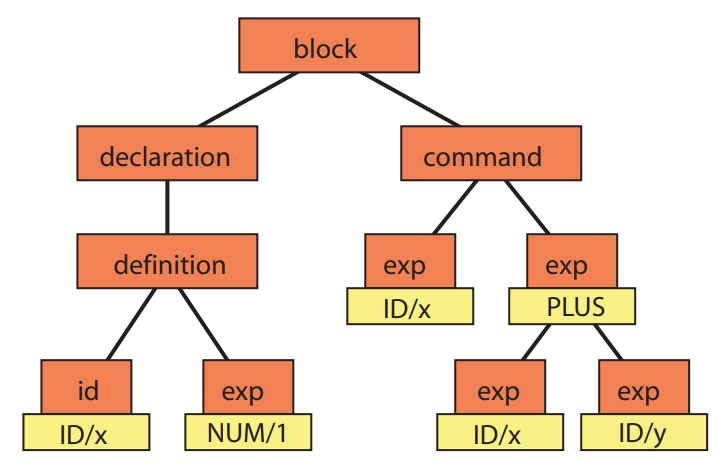
\includegraphics[width=10cm]{parsetree.png}
\end{center}
\subsection{\textcolor{blue}{trans}}
\textbf{Translation} phase flattens the (modified) tree into a linear sequence of \textbf{intermediate code}
\subsection{\textcolor{magenta}{intermediate code}}
This is something like bytecode
\subsection{\textcolor{blue}{cg}}
\textbf{Code Generation} phase converts the intermediate code into \textbf{assembly} and then into \textbf{machine code}. This optimises for the specific processor architecture
\subsection{\textcolor{magenta}{machine code}}
\newpage

\section{Lexical analysis}
A \textbf{regular expression} over some \textbf{alphabet} $\Sigma$ (finite set of symbols)
\begin{itemize}
\item Any a $\in \Sigma$ is a regular expression. A regular expression is any letter from the alphabet
\item $\varnothing$ (empty set) and $\epsilon$ (empty string) are regular expressions
\item If $\omega$ and $\omega'$ are regular expressions then so are:
\begin{itemize}
\item $(\omega\omega')$ - x concatenated with y
\item $(\omega|\omega')$ - Logical or for example $gr|a|e|y$ would fit for both spellings of the colour
\item $(\omega*)$ - 0 or more copies of $\omega$ in a row
\end{itemize}
\end{itemize}
Every regular expression denotes a \textbf{set of strings} (or \textbf{language}) over $\Sigma$

\section{Some regular expressions}
\begin{itemize}
\item Consider defining all strings over $\{a,b\}$ beginning with a and ending in b
\begin{itemize}
\item $a(a|b)^*b$ - a at start and b at end with as many as and bs in the middle as needed
\end{itemize}

\item Consider defining all strings over $\Sigma=\{a,b\}$ containing the string abab
\begin{itemize}
\item $(a|b)^*abab(a|b)^*$
\end{itemize}

\item Consider defining all strings over $\Sigma=\{a,b\}$ where no two a's appear consecutively
\begin{itemize}
\item $(ab|b)^*(a|\epsilon)$
\item $b^*(abb^*)^*(a|\epsilon)$
\item There are different regular expressions that do the same thing, it is a difficult problem to decide whether two regular expressions describe the same set of strings
\end{itemize}

\item Consider defining all strings over $\Sigma=\{a,b,c\}$ where there is an even number of c's
\begin{itemize}
\item $(a|b)^*(c(a|b)^*c(a|b)^*)^*(a|b)^*$
\end{itemize}

\item Regular expressions
\begin{itemize}
\item Found in search engines, word processors, text editors, etc
\item Python provides regular expression support via the module re
\end{itemize}
\end{itemize}

\section{Finite state machines}
A \textbf{finite state machine (FSM)} $M=(\Sigma,Q,\delta:Q\times \Sigma \rightarrow Q, q_0\in Q,F$ where:
\begin{itemize}
\item $\Sigma$ is some finite alphabet
\item Q is a finite set of \textbf{states} with \textbf{initial state} $q_0$ and \textbf{final states} $f\subseteq Q$
\item $\delta: Q\times\Sigma\rightarrow Q$ is a \textbf{transition function}
\end{itemize}
On input a string $a_1,a_2...a_n$ over $\Sigma$, M yields a state sequence $q_0,q_1,...,q_n$ via:
\begin{itemize}
\item $q_1=\delta(q_0,a_1),q_2=\delta(q_1,a_2),...q_n=\delta(q_{n-1},a_n)$
\item $a_1,a_2,...a_n$ is \textbf{accepted} if $q_n\in F$
\end{itemize}
Pictorial representation: The FSM below accepts the set of strings not containing 2 consecutive a's
\begin{center}
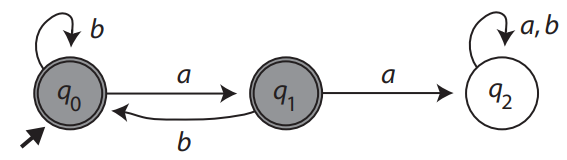
\includegraphics[width=6cm]{FSM1.png}
\end{center}
\textbf{Theorem}: A set of strings is denoted by a regular expression if, and only if, it is accepted by a finite state machine (such sets of strings are called the \textbf{regular languages}
\subsection{Examples}

\subsubsection{Example 1}
\begin{center}
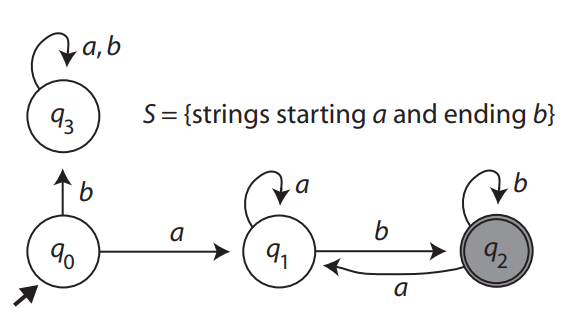
\includegraphics[width=6cm]{FSM2.png}
\end{center}
\subsubsection{Example 2}
\begin{center}
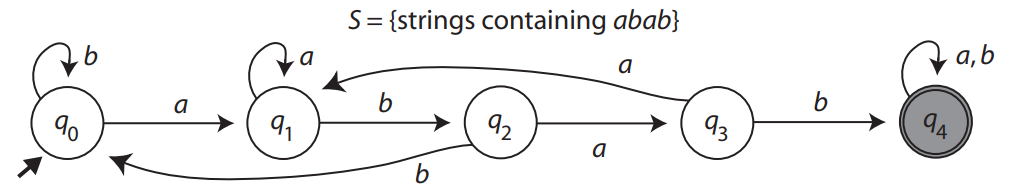
\includegraphics[width=10cm]{FSM3.png}
\end{center}
\subsubsection{Example 3}
\begin{center}
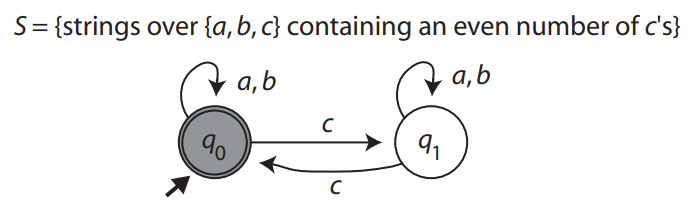
\includegraphics[width=8cm]{FSM4.png}
\end{center}



\section{Syntax analysis}
\begin{itemize}
\item While tokens are defined using regular languages, programming language syntax is almost always describable by a \textbf{context-free grammar}
\item Need to check that what has been written follows the rules of the language
\item Some things not picked up by lexical analysis will be picked up by syntax analysis
\item \textbf{A phase structure grammar} is a four tuple (N,T,s,R) where
\begin{itemize}
\item T and N are disjoint finite sets of \textbf{terminal} and \textbf{non terminal} symbols
\item $s\in N$ is the start symbol 
\item R is a finite set of productions or rules
\end{itemize}
\item In a context free grammar, productions are of the form:
\begin{itemize}
\item $b\rightarrow a_1a_2...a_k \quad$ with $k\geqslant0, b\in N$ and $a_1,a_2,...,a_k\in N\cup T$
\end{itemize}
\end{itemize}
Example: A production $b\rightarrow a_1a_2...a_k$ can be \textbf{applied} to a string $\epsilon$ containing b via:
$$\omega=...b'bb''... \Rightarrow = ...b'a_1a_2...a_kb''$$
\begin{itemize}
\item A grammar \textbf{generates} the set of strings over T that can be obtained by repeatedly applying productions starting from the string s
\item Note that we may have a choice of production to apply; that is, the process is \textbf{non deterministic}
\end{itemize}
\newpage
\section{A context free grammar}
\begin{itemize}
\item Consider the context-free grammar (N=\{s,t,u\}, T=\{a,b\},s,R) with R consisting of the productions:
$$s\rightarrow\epsilon \qquad s\rightarrow bs \qquad s\rightarrow at \qquad t\rightarrow bs \qquad	 t\rightarrow \epsilon \qquad t\rightarrow au$$
\item We start with s; there are 3 choices in which production to apply
\begin{itemize}
\item $s\rightarrow \epsilon$ \qquad \qquad and we are finished having generated $\epsilon$
\item $s\rightarrow bs$
\item $s\rightarrow at$
\end{itemize}
\item Perhaps we repeatedly apply $s\rightarrow bs$:
\begin{itemize}
\item $s\rightarrow bs \rightarrow bbs \rightarrow bbbs \rightarrow...\rightarrow b^ns$
\item And then $s\rightarrow at$ to get $b^nat$, or $s\rightarrow \epsilon$ to finish and generate $b^n$ (where $n\geqslant 1$)
\end{itemize}
\item So, if we haven't finished then we have derived $b^nat$ where $n\geqslant 0$
\item Perhaps we apply $t\rightarrow bs$ to derive $b^nabs$ ... or maybe we apply $t\rightarrow \epsilon$ to generate $b^na$ ... or maybe $t\rightarrow au$ to derive $b^naau$ from whence we are stuck
\item So if we haven't finished or aren't stuck then we've got $b^nabs$: go again
\item Arguing in this way we generate the knowledge that you cannot have 2 consecutive as
\end{itemize}
\section{Regular Grammars}
\begin{itemize}
\item Regular grammars are special types of context-free grammars
\item A \textbf{regular grammar} (N,T,s,R) is a context free grammar where all productions are of one of the following forms
\begin{itemize}
\item $b\rightarrow a$ \qquad \qquad where $a\in T$
\item $b\rightarrow ac$ \qquad \qquad where $a\in T, c\in N$
\item $b\rightarrow \epsilon$
\end{itemize}
\end{itemize}
\subsection{Theorem}
A set of strings is represented by a regular expression if, and only if, it it accepted by a finite state machine if, and only if, it is generated by some regular grammar
\begin{itemize}
\item So, we can build regular grammars generating the earlier sets of string
\item There exist context-free languages that are not regular e.g., $\{a^nb^n: n\geqslant 1\}$
\item There are special machines called \textbf{pushdown automata} that characterize the languages generated by context free grammars
\begin{itemize}
\item essentially, finite state machines equipped with extra memory called a \textbf{stack}
\end{itemize}
\item If the syntax of a programming languages can be described using a context free grammar then it turns out that we can quickly build parse trees and so efficiently spot programs that are incorrectly written
\end{itemize}
\section{Backus Naur Form}
\begin{itemize}
\item In the world of programming languages, context free grammars are usually expressed in \textbf{Backus Naur Form (BNF)}:
\begin{itemize}
\item Productions with the same left hand sides can be separated with $|$
\item non-terminals appear inside $<>$
\item ::= is used instead of $\rightarrow$
\end{itemize}
\end{itemize}







Uses ::= instead of $\rightarrow$\\
Non terminals appear inside $<>$\\
\\
For example $s\rightarrow at$ would become $<s>::=a<t>$

\end{document}